\section{System Architecture Overview}

This section provides an overview of the architecture of our indoor navigation system, designed to assist visually impaired users with real-time, context-aware guidance within indoor environments. The system leverages mobile technology, backend services, and sensory input devices to deliver seamless and accessible navigation. Below, we briefly introduce the key components and their roles, supported by a use case diagram and system architecture illustration.

\subsection{High-Level View of Components}

The system comprises four main components, each explained briefly below. Detailed descriptions of each component are provided in subsequent sections.

\begin{itemize}
	\item \textbf{Mobile Application}: The mobile application acts as the central interface for users and the processing unit for the system. It facilitates QR code scanning, provides navigation instructions via TalkBack, processes obstacle detection data, and communicates with the backend server to retrieve location-specific data. The app also enables users to connect the IO components they want. This is done by choosing th desired camera, microphone, and sound output devices from the settings. The default devices will be the ones on the phone.
	
	\item \textbf{Localization System}: The localization system determines the user’s global position and orientation within the environment. It uses QR code scanning and positional data retrieval from the backend to calculate the user’s current position relative to the environment.
	
	\item \textbf{Customizable Guidance System}: The guidance system provides real-time navigation assistance by retrieving and delivering location-based instructions. It allows users to select destinations and offers step-by-step guidance through TalkBack, dynamically updating as the user progresses along the path.
	
	\item \textbf{Obstacle Detection System}: The obstacle detection system ensures safety by alerting users to nearby obstacles. Using four ultrasonic sensors and vibration motors, it delivers tactile feedback proportional to the proximity of detected obstacles, enhancing the user's awareness of their surroundings.


	\item \textbf{Building Management Dashboard}: The Building Management Dashboard provides secure authentication for administrators to access and manage their building layouts, including all QR codes within the building. It allows them to edit instructions, generate printable QR codes, and perform bulk updates to instructions across a floor, section, or the entire building efficiently.
	
\end{itemize}

\subsection{Constraints and Standards}

During the design and implementation of the Mosaned system, several constraints and standards were considered to ensure feasibility, compatibility, usability, and compliance with best practices.

\subsubsection{Constraints}

\begin{itemize}
	\item \textbf{Hardware Constraints:} The system was constrained by the need to use low-cost and widely available components, such as the ESP32 microcontroller, HC-SR04 ultrasonic sensor, and C1026B coin vibration motor. This influenced performance capabilities, especially in processing and communication speed.
	
	\item \textbf{Power Constraints:} The wearable nature of the system necessitated low power consumption. All hardware components were selected and configured to optimize battery life.
	
	\item \textbf{Environmental Constraints:} The system had to operate under varying lighting conditions and within different indoor layouts. Robustness to light variations was achieved through camera calibration and reliable QR code detection.
	
	\item \textbf{User Constraints:} Since the target users are visually impaired individuals, the system was designed with minimal manual input, using accessible Android features like TalkBack and haptic feedback for interaction.
	
	\item \textbf{Connectivity Constraints:} Some features such as downloading building metadata required an internet connection only once. Thereafter, offline functionality was mandatory to support real-world usage without dependency on constant connectivity.
	
	\item \textbf{Deployment Constraints:} QR code placement within buildings needed standardization to ensure consistent detection. A uniform placement policy (e.g., on walls or hanging panels at a consistent height) was considered essential.
\end{itemize}

\subsubsection{Standards}

\begin{itemize}
	\item \textbf{QR Code Standards:} The system complies with ISO/IEC 18004:2015 standards for QR code structure and encoding, ensuring compatibility with open-source libraries like ZXing and OpenCV.
	
	\item \textbf{Accessibility Standards:} The mobile application adheres to Android Accessibility Guidelines, incorporating TalkBack compatibility, high contrast UI, and minimal touch navigation.
	
	
	\item \textbf{Communication Protocols:} Bluetooth Low Energy (BLE) was used for connecting the ESP32 modules, complying with Bluetooth specifications to ensure interoperability and low power consumption.
	
	\item \textbf{Data Privacy and Security:} The management dashboard uses secure user authentication (e.g., hashed passwords) and access control, ensuring that only authorized administrators manage building data.
\end{itemize}

These constraints and standards were foundational in shaping a system that is not only functional and user-centered but also practical for deployment and scaling.



\subsection{System Architecture Diagram}

The system architecture diagram (see Figure~\ref{fig:system_architecture}) provides a high-level view of how the components are connected and interact, where the arrows show the flow of data. 

\begin{figure}[h]
	\centering
	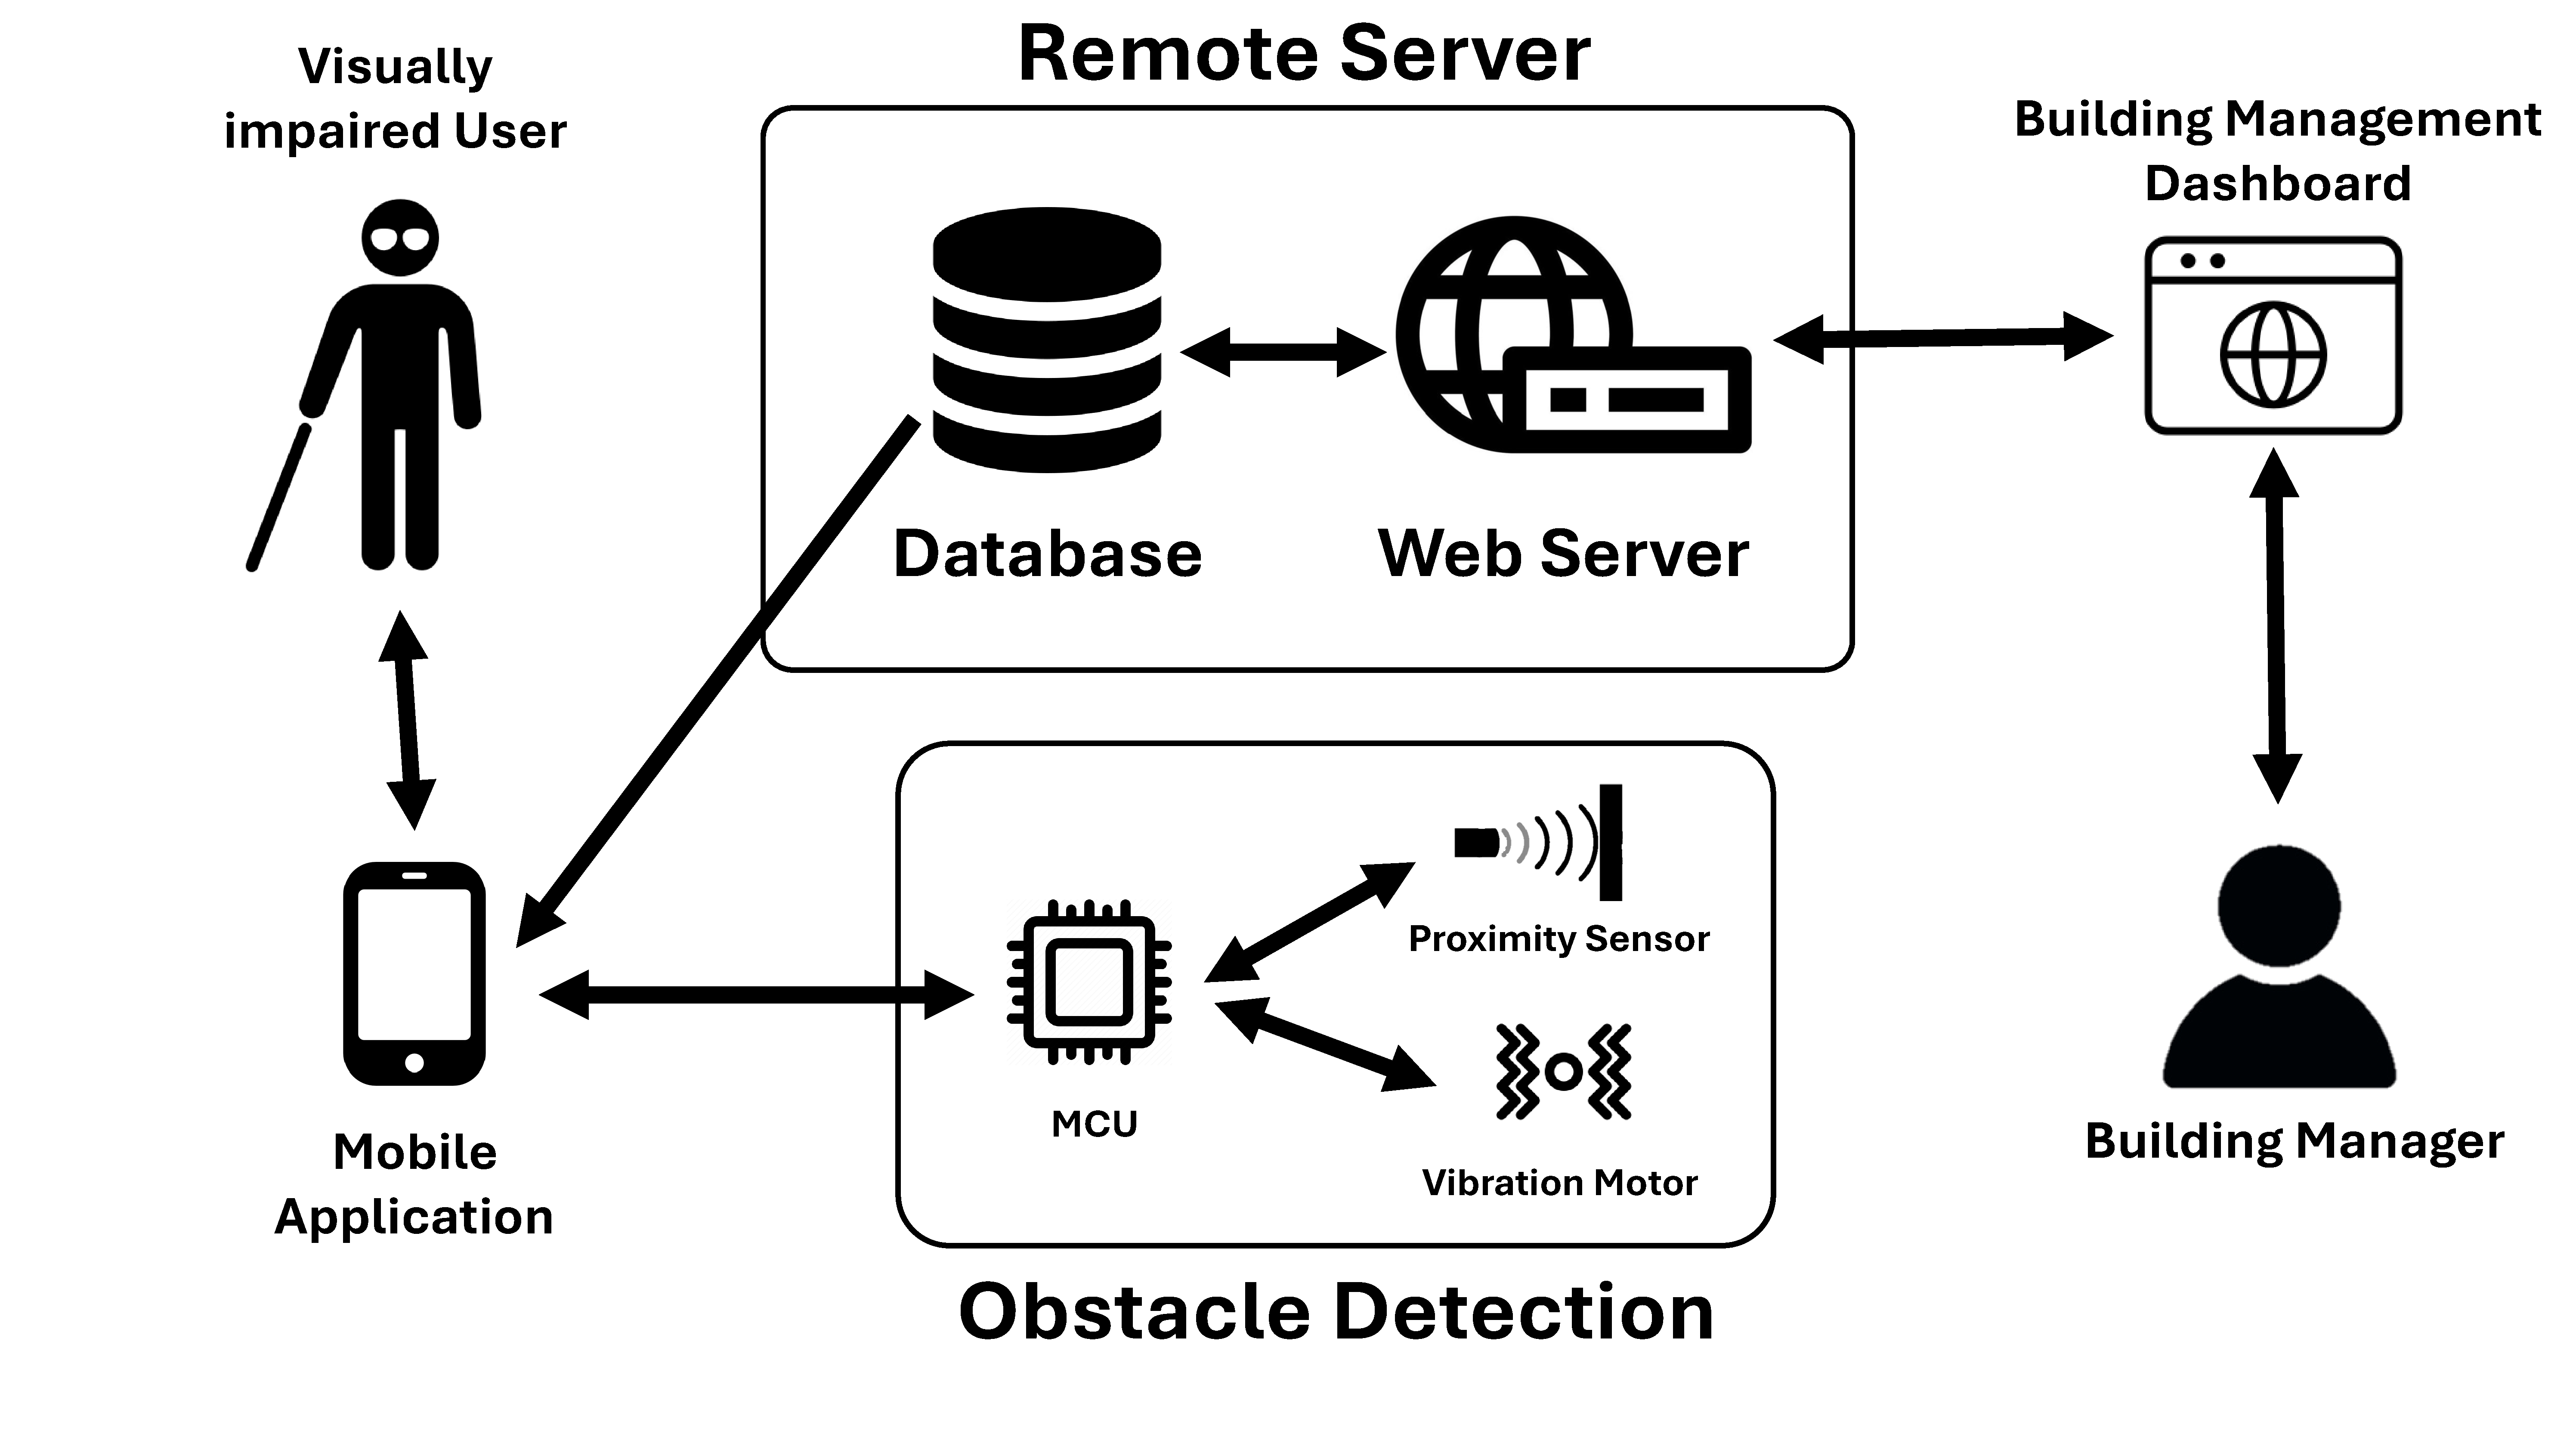
\includegraphics[width=1\linewidth]{assets/ch2/sys_arch}
	\caption{System Architecture Diagram of Mosaned System}
	\label{fig:system_architecture}
\end{figure}

This high-level overview introduces the core components and their functions within the system. Subsequent sections provide detailed explanations of each component, their implementation, and integration.
